% EDC_Neutron_Junction_Model.tex
% Companion N to Paper 3: Neutron as Excited 5D Junction
% Version 0.1 (Draft) — 2026-01-20
% Build: XeLaTeX (Unicode)

\documentclass[11pt,a4paper]{article}

% ============================================================
%  PACKAGES
% ============================================================
\usepackage{fontspec}
\usepackage{amsmath,amssymb,amsthm}
\usepackage{mathtools}
\usepackage{physics}
\usepackage{geometry}

% FONTS (TeX Gyre Termes = Times-like with full OpenType support)
\IfFontExistsTF{TeX Gyre Termes}{%
  \setmainfont{TeX Gyre Termes}
  \setsansfont{TeX Gyre Heros}
}{%
  \setmainfont{Times New Roman}[Ligatures=TeX]
  \setsansfont{Helvetica}
}
\geometry{margin=2.5cm}
\usepackage{hyperref}
\hypersetup{
    colorlinks=true,
    linkcolor=blue,
    citecolor=blue,
    urlcolor=blue,
    pdfborder={0 0 0}
}
\usepackage{enumitem}
\usepackage{booktabs}
\usepackage{array}
\usepackage{xcolor}
\usepackage{tcolorbox}
\usepackage{tikz}
\usetikzlibrary{calc,angles,quotes,decorations.markings,decorations.pathmorphing}
\usepackage{gensymb}

% ============================================================
%  EPISTEMIC TAG COMMANDS
% ============================================================
\definecolor{tagDer}{RGB}{0,128,0}      % Green - Derived
\definecolor{tagDc}{RGB}{0,0,200}       % Blue - Deduced/Constrained
\definecolor{tagCal}{RGB}{200,0,0}      % Red - Calibrated
\definecolor{tagP}{RGB}{128,0,128}      % Purple - Postulated
\definecolor{tagBL}{RGB}{128,128,128}   % Gray - Baseline
\definecolor{tagI}{RGB}{255,140,0}      % Orange - Identified
\definecolor{tagOpen}{RGB}{200,100,0}   % Dark orange - Open

\newcommand{\tagDer}{\textcolor{tagDer}{\textbf{[Der]}}}
\newcommand{\tagDc}{\textcolor{tagDc}{\textbf{[Dc]}}}
\newcommand{\tagCal}{\textcolor{tagCal}{\textbf{[Cal]}}}
\newcommand{\tagP}{\textcolor{tagP}{\textbf{[P]}}}
\newcommand{\tagBL}{\textcolor{tagBL}{\textbf{[BL]}}}
\newcommand{\tagI}{\textcolor{tagI}{\textbf{[I]}}}
\newcommand{\tagOpen}{\textcolor{tagOpen}{\textbf{[OPEN]}}}
\newcommand{\tagDef}{\textcolor{tagDc}{\textbf{[Def]}}}

% ============================================================
%  THEOREM ENVIRONMENTS
% ============================================================
\newtheorem{postulate}{Postulate}
\newtheorem{definition}{Definition}[section]
\newtheorem{theorem}{Theorem}[section]
\newtheorem{lemma}[theorem]{Lemma}
\newtheorem{corollary}[theorem]{Corollary}
\newtheorem{proposition}[theorem]{Proposition}
\newtheorem{remark}{Remark}[section]

% ============================================================
%  CUSTOM COMMANDS
% ============================================================
\newcommand{\re}{r_e}
\newcommand{\Ztwo}{\mathbb{Z}_2}
\newcommand{\Ztri}{\mathbb{Z}_3}
\newcommand{\Zthree}{\mathbb{Z}_3}
\newcommand{\Zsix}{\mathbb{Z}_6}
\newcommand{\Sthree}{S^3}
\newcommand{\Stwo}{S^2}
\newcommand{\Bthree}{B^3}
\newcommand{\Mfive}{\mathcal{M}_5}
\newcommand{\Bfour}{\mathcal{B}_4}
\newcommand{\tension}{\tau}  % string/flux-tube tension (E/L)

% ============================================================
%  TITLE
% ============================================================
\title{\textbf{Neutron as Excited 5D Junction}\\[0.3em]
\Large in Elastic Diffusive Cosmology\\[0.5em]
\normalsize (Companion N to Paper~3: NJSR Edition)\\[0.3em]
\footnotesize Draft v0.1 (January 2026)}
\author{Igor Gr\v{c}man}
\date{January 2026\\[0.5em]
\small DOI: \href{https://doi.org/10.5281/zenodo.18315110}{10.5281/zenodo.18315110}\\[0.3em]
\small Repository: \href{https://github.com/igorgrcman/elastic-diffusive-cosmology}{github.com/igorgrcman/elastic-diffusive-cosmology}\\[0.2em]
\footnotesize (Public artifacts for this paper are in the \texttt{edc\_papers} folder.)}

% ============================================================
%  DOCUMENT
% ============================================================
\begin{document}

\maketitle

% ------------------------------------------------------------
%  RELATED DOCUMENTS
% ------------------------------------------------------------
\begin{center}
\small\textbf{Related Documents:}\\[0.1cm]
\footnotesize
\emph{Neutron Lifetime from 5D Membrane Cosmology} (DOI: \href{https://doi.org/10.5281/zenodo.18262721}{10.5281/zenodo.18262721})\\[0.05cm]
\emph{Framework v2.0} (DOI: \href{https://doi.org/10.5281/zenodo.18299085}{10.5281/zenodo.18299085})\\[0.05cm]
\textbf{Companions:}\\
A: \emph{Effective Lagrangian} (\href{https://doi.org/10.5281/zenodo.18292841}{DOI}) ~$\cdot$~
B: \emph{WKB Prefactor} (\href{https://doi.org/10.5281/zenodo.18299637}{DOI})\\
C: \emph{5D Reduction} (\href{https://doi.org/10.5281/zenodo.18299751}{DOI}) ~$\cdot$~
D: \emph{Selection Rules} (\href{https://doi.org/10.5281/zenodo.18299855}{DOI})\\
E: \emph{Symmetry Ops} (\href{https://doi.org/10.5281/zenodo.18300199}{DOI}) ~$\cdot$~
F: \emph{Proton Junction} (\href{https://doi.org/10.5281/zenodo.18302953}{DOI})\\
G: \emph{Mass Difference} (\href{https://doi.org/10.5281/zenodo.18303494}{DOI}) ~$\cdot$~
H: \emph{Weak Interactions} (\href{https://doi.org/10.5281/zenodo.18307539}{DOI})\\[0.05cm]
\textbf{This:} N: \emph{Neutron Junction} (\href{https://doi.org/10.5281/zenodo.18315110}{DOI})
\end{center}

% ------------------------------------------------------------
%  ABSTRACT
% ------------------------------------------------------------
\begin{abstract}
We establish the neutron as an \textbf{excited 5D junction state} within Elastic Diffusive Cosmology (EDC). The neutron shares the same three-arm junction topology as the proton (Companion F), but is displaced from the local Steiner minimum---the universal $120\degree$ optimum in the tangent metric. This excitation couples to the bulk-facing side of a thick brane, pumping energy into brane-layer modes. The observer-side frozen projection boundary then organizes the released energy into allowed weak-channel outputs ($e^- + \bar{\nu}_e$).

\textbf{Calibration boundary:} The neutron lifetime $\tau_n \approx 879\,\text{s}$ is treated as a \textbf{baseline observable} \tagBL{}, not as a prediction of this companion. The lifetime value enters only as a phenomenological check; no parameters are fitted to it here.

\textbf{Epistemic status:} The junction postulate is \tagP{} (inherited from Companion F). Given this postulate, the neutron's excited nature is \tagP{}, while the Steiner relaxation mechanism is \tagDc{}. The thick-brane pumping and frozen projection remain \tagOpen{} at the microphysics level.
\end{abstract}

\tableofcontents

\vspace{1em}
\begin{tcolorbox}[colback=blue!5,colframe=blue!40!black,title=\textbf{Cornerstone: Neutron in EDC}]
In the EDC program, the neutron is modeled as an excited 5D junction state: the same three-arm junction core as the proton, but displaced from the local Steiner minimum (the universal $120\degree$ optimum in the tangent metric). This excitation couples to the bulk-facing side of a thick brane, pumping energy into brane-layer modes. The observer-side frozen projection boundary then organizes the released energy into allowed weak-channel outputs (e.g., $e^-$ and $\bar{\nu}_e$), while overall bulk--brane conservation remains anchored to Framework v2.0, Remark~4.5.

\medskip
\textbf{Epistemic status:}
\begin{itemize}[nosep]
    \item $120\degree$ as local optimum: \tagDer{}/\tagDc{} (geometric, from Companion F)
    \item Neutron = excited junction: \tagP{} (object assumption)
    \item Thick-brane pumping + frozen output mapping: \tagP{}/\tagOpen{}
\end{itemize}
\end{tcolorbox}

\newpage

% ============================================================
%  SECTION 1: MOTIVATION AND SCOPE
% ============================================================
\section{Motivation and Scope}
\label{sec:motivation}

\subsection{The Gap: Neutron Object Model}

Companion F establishes the proton as a Y-junction in 5D---a three-arm flux-tube network meeting at $120\degree$ angles (Steiner configuration). Companion G derives the neutron-proton mass difference from $\Zsix$ symmetry breaking. Companion H describes weak interactions as junction transitions mediated by thick-brane microphysics.

\textbf{What is missing:} A clear statement of \emph{what the neutron is} as a 5D object, analogous to Companion F's treatment of the proton.

\subsection{Purpose of This Companion}

This document provides the \textbf{neutron backbone}:
\begin{enumerate}
    \item Define the neutron as an excited 5D junction state \tagP{}
    \item Show that instability arises from displacement from Steiner minimum \tagDc{}
    \item Connect junction oscillation to thick-brane energy pumping \tagP{}/\tagOpen{}
    \item Describe the frozen projection boundary as organizing outputs \tagDc{}/\tagP{}
    \item Identify the bridge to Paper 3's WKB treatment \tagOpen{}
\end{enumerate}

\subsection{What This Companion Does NOT Do}

\begin{itemize}
    \item Does NOT derive the lifetime $\tau_n \approx 879\,\text{s}$ from first principles (remains \tagCal{} via Paper 3's WKB barrier)
    \item Does NOT derive the V--A structure of weak interactions (Standard Model input \tagBL{})
    \item Does NOT derive the thick-brane coupling constant (remains \tagOpen{})
\end{itemize}

\subsection{Epistemic Hierarchy}

\begin{center}
\begin{tabular}{lll}
\toprule
\textbf{Level} & \textbf{Content} & \textbf{Status} \\
\midrule
Inherited & Baryon = 3-arm junction in 5D bulk & \tagP{} (from F) \\
Inherited & Equal tensions $\Rightarrow$ $120\degree$ angles & \tagDer{} (from F) \\
Postulate & Neutron = excited (non-Steiner) junction & \tagP{} \\
Definition & Collective coordinate $q = |\hat{e}_1 + \hat{e}_2 + \hat{e}_3|/3$ & \tagDef{} \\
Consequence & Excitation carries geometric energy & \tagDc{} \\
Model & Ring mode + 3 springs (heuristic) & \tagI{}/\tagP{} \\
Open & Thick-brane pumping mechanism & \tagOpen{} \\
Open & WKB--damping bridge & \tagOpen{} \\
\bottomrule
\end{tabular}
\end{center}

% ============================================================
%  SECTION 2: THICK-BRANE SETTING
% ============================================================
\section{Thick-Brane Setting}
\label{sec:thick-brane}

This section summarizes the thick-brane framework established in Companion H. The brane is not a mathematical surface but a \textbf{finite-thickness layer} with distinct bulk-facing and observer-facing boundaries.

\subsection{The Brane as ``Glass Window''}

\begin{tcolorbox}[colback=yellow!5,colframe=orange!50!black,title=\textbf{Conceptual Picture \tagP}]
\begin{center}
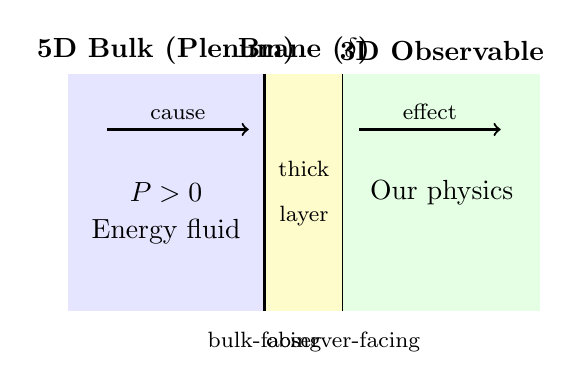
\begin{tikzpicture}[scale=1.0]
    % Bulk side
    \fill[blue!10] (-3,-1.5) rectangle (-0.5,1.5);
    \node at (-1.75,1.8) {\textbf{5D Bulk (Plenum)}};
    \node at (-1.75,0) {$P > 0$};
    \node at (-1.75,-0.5) {Energy fluid};

    % Brane
    \fill[yellow!20] (-0.5,-1.5) rectangle (0.5,1.5);
    \draw[very thick] (-0.5,-1.5) -- (-0.5,1.5);
    \draw[very thick] (0.5,-1.5) -- (0.5,1.5);
    \node at (0,1.8) {\textbf{Brane ($\delta$)}};
    \node[font=\footnotesize] at (0,0.3) {thick};
    \node[font=\footnotesize] at (0,-0.3) {layer};

    % Observer side
    \fill[green!10] (0.5,-1.5) rectangle (3,1.5);
    \node at (1.75,1.8) {\textbf{3D Observable}};
    \node at (1.75,0) {Our physics};

    % Labels
    \node[font=\footnotesize] at (-0.5,-1.9) {bulk-facing};
    \node[font=\footnotesize] at (0.5,-1.9) {observer-facing};

    % Arrows
    \draw[->,thick] (-2.5,0.8) -- (-0.7,0.8) node[midway,above,font=\footnotesize] {cause};
    \draw[->,thick] (0.7,0.8) -- (2.5,0.8) node[midway,above,font=\footnotesize] {effect};
\end{tikzpicture}
\end{center}

\textbf{Key idea:} The brane has TWO sets of boundary conditions:
\begin{itemize}[nosep]
    \item \textbf{Left (bulk-facing):} BC toward 5D bulk (Plenum, energy fluid)
    \item \textbf{Right (observer-facing):} BC toward 3D observable universe (our physics)
\end{itemize}
Physics in 5D is the \textbf{cause}; 3D observations are the \textbf{effect}.
\end{tcolorbox}

\subsection{Bulk--Brane Energy Exchange}

\begin{remark}[Canonical reference \textup{\tagBL}]
\label{rem:energy-exchange}
See Framework v2.0, Remark~4.5 for the canonical bulk--brane conservation statement and sign convention ($J^\nu_{\text{bulk}\to\text{brane}} > 0$ = INFLOW).
\end{remark}

The thick-brane allows energy to flow from bulk structures (junctions) into brane-localized modes, which then appear as observable particles on the 3D side.

\subsection{Frozen Projection Boundary}

\begin{definition}[Frozen Projection \textup{\tagDc}/\textup{\tagP}]
\label{def:frozen-projection}
The \textbf{frozen projection boundary} is the observer-facing interface where:
\begin{enumerate}[nosep]
    \item High-frequency bulk modes are adiabatically eliminated (``frozen'')
    \item Only allowed channels (selection rules) can carry energy to 3D
    \item Acts as a \textbf{one-way valve}: INFLOW allowed, OUTFLOW suppressed
\end{enumerate}
\end{definition}

For neutron decay, this boundary organizes the released junction energy into the $\beta^-$ channel: $e^- + \bar{\nu}_e + \text{recoil}$.

% ============================================================
%  SECTION 3: NEUTRON AS EXCITED JUNCTION
% ============================================================
\section{Neutron as Excited Junction: Ontology}
\label{sec:ontology}

\subsection{Same Topology, Different State}

\begin{postulate}[Neutron as Excited Junction \textup{\tagP}]
\label{post:neutron-excited}
In 5D EDC, the neutron is a three-arm flux-tube junction with the \textbf{same topological structure} as the proton, but in an \textbf{excited state}---displaced from the Steiner minimum.
\end{postulate}

\begin{center}
\begin{tabular}{lcc}
\toprule
& \textbf{Proton} & \textbf{Neutron} \\
\midrule
Topology & Y-junction (3 arms) & Y-junction (3 arms) \\
Arm angles & $120\degree$ (Steiner) & $\neq 120\degree$ (excited) \\
Energy state & Ground state (minimum) & Metastable (excited) \\
Stability & Stable & Unstable ($\tau \approx 879$ s) \\
Charge (Q) & +1 & 0 \\
\bottomrule
\end{tabular}
\end{center}

\subsection{Collective Coordinate}

\begin{definition}[Collective Coordinate $q$ \textup{\tagDef}]
\label{def:collective-q}
Let $\hat{e}_i$ ($i = 1,2,3$) be the unit tangent vectors at the junction. The collective coordinate measuring departure from Steiner symmetry is:
\begin{equation}
\boxed{q \equiv \frac{1}{3}\left| \hat{e}_1 + \hat{e}_2 + \hat{e}_3 \right|}
\label{eq:q-def}
\end{equation}
\end{definition}

\begin{proposition}[Range and Interpretation \textup{\tagDer}]
\label{prop:q-range}
The collective coordinate satisfies:
\begin{itemize}
    \item $q = 0$: Steiner configuration ($\hat{e}_1 + \hat{e}_2 + \hat{e}_3 = 0$) $\Rightarrow$ \textbf{proton}
    \item $q = 1$: Maximal asymmetry (all arms parallel) $\Rightarrow$ unphysical limit
    \item $0 < q < 1$: Excited states, including \textbf{neutron}
\end{itemize}
\end{proposition}

\begin{proof}
For unit vectors summing to zero (Steiner), $|\sum \hat{e}_i| = 0$, hence $q = 0$. For all parallel, $|\sum \hat{e}_i| = 3$, hence $q = 1$. Intermediate configurations give $0 < q < 1$.
\end{proof}

\begin{remark}[Neutron value of $q$ \textup{\tagI}/\textup{\tagOpen}]
\label{rem:q-neutron}
Based on $\Zsix$ symmetry arguments (Companion G), the neutron corresponds to approximately:
\begin{equation}
q_n \approx \frac{1}{3} \quad \text{(or equivalently, half-Steiner displacement)}
\end{equation}
The precise value and its derivation from first principles remain \tagOpen{}. Current estimates give $q_n \approx 0.31$ from phenomenological matching.
\end{remark}

\subsection{Energy from Displacement}

\begin{lemma}[Geometric Excitation Energy \textup{\tagDc}]
\label{lem:excitation-energy}
Any displacement from the Steiner minimum ($q = 0$) carries positive geometric energy:
\begin{equation}
E_{\text{geom}}(q) = E_0 + \kappa_q \, q^2 + O(q^4)
\label{eq:energy-taylor}
\end{equation}
where $\kappa_q > 0$ is the stiffness of the junction against asymmetric deformations.
\end{lemma}

\begin{proof}
The Steiner point is a local minimum of the total weighted length (Companion F, Theorem 4.1). Near a minimum, the energy expands as a positive-definite quadratic form to leading order.
\end{proof}

\begin{corollary}[Instability \textup{\tagDc}]
The neutron ($q_n > 0$) has higher energy than the proton ($q = 0$). This energy difference drives relaxation toward the Steiner minimum.
\end{corollary}

\begin{figure}[h]
\centering
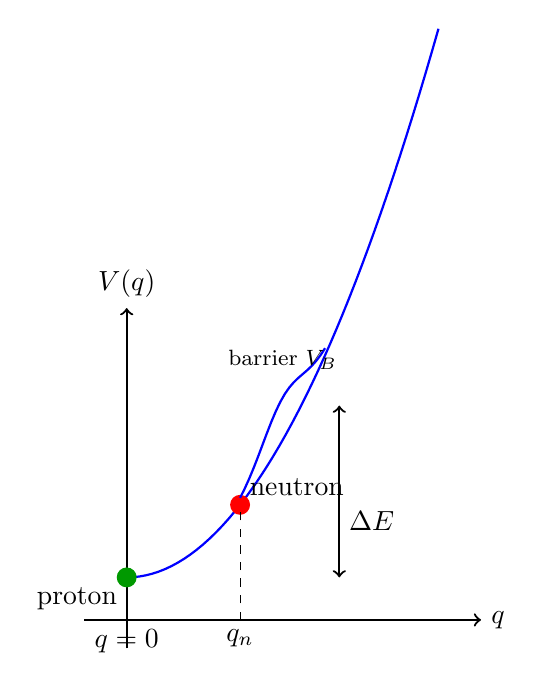
\begin{tikzpicture}[scale=1.8]
    % Potential well
    \draw[thick,->] (-0.3,0) -- (2.5,0) node[right] {$q$};
    \draw[thick,->] (0,-0.2) -- (0,2.2) node[above] {$V(q)$};

    % Potential curve
    \draw[thick,blue,domain=0:2.2,samples=50] plot (\x, {0.3 + 0.8*\x*\x});

    % Proton minimum
    \fill[green!60!black] (0,0.3) circle (2pt);
    \node[below left] at (0,0.3) {proton};
    \node[below] at (0,0) {$q=0$};

    % Neutron excited
    \fill[red] (0.8,0.812) circle (2pt);
    \node[above right] at (0.8,0.812) {neutron};
    \draw[dashed] (0.8,0) -- (0.8,0.812);
    \node[below] at (0.8,0) {$q_n$};

    % Energy difference
    \draw[<->,thick] (1.5,0.3) -- (1.5,0.812+0.7);
    \node[right] at (1.5,0.7) {$\Delta E$};

    % Barrier (schematic)
    \draw[thick,blue,domain=0.8:1.4,samples=20] plot (\x, {0.3 + 0.8*\x*\x + 0.3*exp(-20*(\x-1.1)*(\x-1.1))});
    \node[above,font=\footnotesize] at (1.1,1.7) {barrier $V_B$};
\end{tikzpicture}
\caption{Schematic potential $V(q)$ for the junction coordinate. The proton sits at $q=0$ (Steiner minimum); the neutron at $q_n > 0$ (metastable excited state). A barrier $V_B$ separates neutron from proton, determining the tunneling lifetime.}
\label{fig:potential}
\end{figure}

% ============================================================
%  SECTION 4: MECHANICS PICTURE
% ============================================================
\section{Mechanics Picture: Ring + 3 Springs}
\label{sec:mechanics}

\subsection{Heuristic Model}

To build intuition for the junction dynamics, we introduce a mechanical analogy.

\begin{tcolorbox}[colback=green!5,colframe=green!40!black,title=\textbf{Mechanical Analogy \tagI/\tagP}]
\textbf{Ring + 3 Springs Model:}

Consider a circular ring of radius $R$ with three springs attached at angles $\theta_1, \theta_2, \theta_3$, each pulling toward the center with spring constant $k$. The springs represent flux-tube tensions; the ring represents a collective constraint.

\medskip
\begin{center}
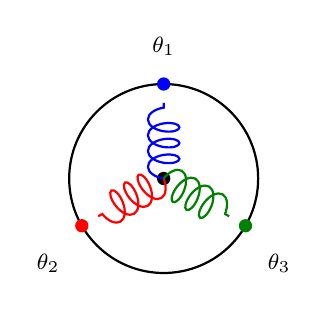
\begin{tikzpicture}[scale=1.2]
    % Ring
    \draw[thick] (0,0) circle (1);

    % Junction center
    \fill (0,0) circle (2pt);

    % Three springs at 120 degrees (equilibrium)
    \foreach \angle/\col in {90/blue, 210/red, 330/green!50!black} {
        \draw[thick,\col,decorate,decoration={coil,aspect=0.5,segment length=2mm,amplitude=2mm}]
            (0,0) -- (\angle:0.8);
        \fill[\col] (\angle:1) circle (2pt);
    }

    % Angles
    \node[above,font=\footnotesize] at (0,1.2) {$\theta_1$};
    \node[below left,font=\footnotesize] at (-1,-0.7) {$\theta_2$};
    \node[below right,font=\footnotesize] at (1,-0.7) {$\theta_3$};
\end{tikzpicture}
\end{center}

\textbf{Interpretation:}
\begin{itemize}[nosep]
    \item Equilibrium: $\theta_1 = \theta_2 = \theta_3 = 120\degree$ (proton)
    \item Excited: angles deviate, springs store extra energy (neutron)
    \item Ring constraint couples all three modes (collective dynamics)
\end{itemize}
\end{tcolorbox}

\subsection{Three-Mode Decomposition}

The junction has three angular degrees of freedom $(\theta_1, \theta_2, \theta_3)$ subject to $\theta_1 + \theta_2 + \theta_3 = 2\pi$. This leaves two independent modes:

\begin{definition}[Mode Decomposition \textup{\tagDef}]
\label{def:modes}
\begin{align}
q &= \text{(collective asymmetry)} = \frac{1}{3}|\hat{e}_1 + \hat{e}_2 + \hat{e}_3| \tag{radial} \\
\perp_1, \perp_2 &= \text{(transverse modes)} \tag{angular}
\end{align}
The collective coordinate $q$ measures overall departure from Steiner; the transverse modes $\perp_{1,2}$ describe shape distortions at fixed $q$.
\end{definition}

\begin{remark}[Effective 1D dynamics \textup{\tagI}]
For slow (adiabatic) relaxation, the transverse modes equilibrate quickly, and the effective dynamics is one-dimensional in $q$. This justifies the 1D WKB treatment in Paper 3.
\end{remark}

\subsection{Linearized Oscillation}

Near the metastable neutron configuration $q = q_n$, the dynamics linearizes to:

\begin{equation}
\ddot{q} + 2\gamma \dot{q} + \omega_0^2 (q - q_n) = 0
\label{eq:damped-oscillator}
\end{equation}

where:
\begin{itemize}
    \item $\omega_0$ = natural frequency (junction stiffness) \tagP{}
    \item $\gamma$ = effective damping (energy loss to brane modes) \tagOpen{}
\end{itemize}

\begin{remark}[Not a Standard Model oscillator \textup{\tagI}]
Equation~\eqref{eq:damped-oscillator} is a \textbf{mechanical linearization} around a geometric minimum---not a quantum field theory oscillator. It captures the qualitative behavior: the junction oscillates around its metastable position while losing energy to the brane.
\end{remark}

% ============================================================
%  SECTION 5: PUMPING AND DISSIPATION
% ============================================================
\section{Pumping and Dissipation Pathway}
\label{sec:pumping}

\subsection{Bulk-Core to Brane-Layer Coupling}

As the junction oscillates/relaxes, it couples to modes within the brane layer:

\begin{tcolorbox}[colback=purple!5,colframe=purple!40!black,title=\textbf{Energy Pathway \tagP/\tagOpen}]
\begin{center}
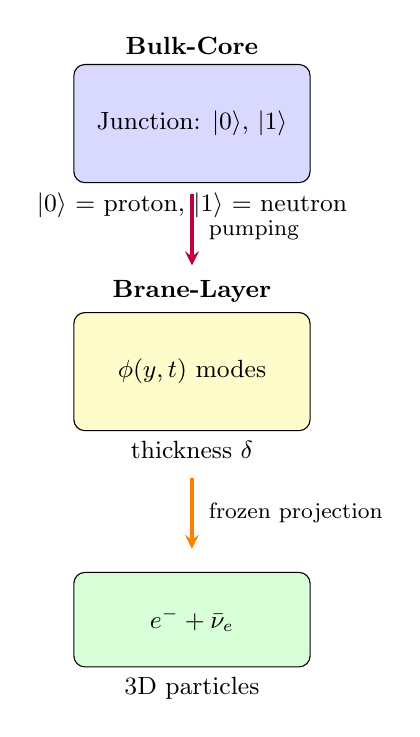
\begin{tikzpicture}[scale=0.9, >=stealth]
    % Bulk core
    \node[draw, rounded corners, fill=blue!15, minimum width=3cm, minimum height=1.5cm] (bulk) at (0,0) {};
    \node[above] at (bulk.north) {\small\textbf{Bulk-Core}};
    \node at (0,0) {\small Junction: $|0\rangle$, $|1\rangle$};
    \node[below,font=\footnotesize] at (bulk.south) {\small $|0\rangle$ = proton, $|1\rangle$ = neutron};

    % Arrow down
    \draw[->,very thick,purple] (0,-1) -- (0,-2);
    \node[right,font=\footnotesize] at (0.1,-1.5) {pumping};

    % Brane layer
    \node[draw, rounded corners, fill=yellow!20, minimum width=3cm, minimum height=1.5cm] (brane) at (0,-3.5) {};
    \node[above] at (brane.north) {\small\textbf{Brane-Layer}};
    \node at (0,-3.5) {\small $\phi(y,t)$ modes};
    \node[below,font=\footnotesize] at (brane.south) {\small thickness $\delta$};

    % Arrow down
    \draw[->,very thick,orange] (0,-5) -- (0,-6);
    \node[right,font=\footnotesize] at (0.1,-5.5) {frozen projection};

    % 3D outputs
    \node[draw, rounded corners, fill=green!15, minimum width=3cm, minimum height=1.2cm] (out) at (0,-7) {};
    \node at (0,-7) {\small $e^- + \bar{\nu}_e$};
    \node[below,font=\footnotesize] at (out.south) {\small 3D particles};
\end{tikzpicture}
\end{center}

\textbf{Mechanism (schematic):}
\begin{enumerate}[nosep]
    \item Neutron junction relaxes: $q_n \to 0$ (toward proton)
    \item Relaxation couples to brane-layer fields: $\mathcal{L}_{\text{int}} \sim g \cdot q(t) \cdot \phi(y=-\delta/2, t)$
    \item Brane modes cascade to observer-facing boundary
    \item Frozen projection selects allowed outputs: $e^- + \bar{\nu}_e + \text{recoil}$
\end{enumerate}
\end{tcolorbox}

\subsection{Coupling Structure}

\begin{postulate}[Bulk-Brane Coupling \textup{\tagP}]
\label{post:coupling}
The junction coordinate $q$ couples linearly to brane-layer modes $\phi$ at the bulk-facing boundary:
\begin{equation}
\mathcal{L}_{\text{int}} = g \, q(t) \, \phi(y = -\delta/2, t)
\label{eq:coupling}
\end{equation}
where $g$ is an effective coupling constant (dimensions and magnitude \tagOpen{}).
\end{postulate}

\begin{remark}[Coupling derivation \textup{\tagOpen}]
\label{rem:coupling-open}
The coupling Eq.~\eqref{eq:coupling} is postulated based on locality (junction at bulk-facing boundary) and linearity (leading-order expansion). A first-principles derivation from the 5D action remains open.
\end{remark}

\subsection{Conservation Ledger}

\begin{remark}[Energy closure \textup{\tagBL}]
Energy released by junction relaxation ($\Delta E = E(q_n) - E(0) \approx \Delta m_{np} c^2 \approx 1.293$ MeV) is transferred to brane modes and ultimately to 3D particles. Total energy is conserved via Framework v2.0, Remark~4.5.
\end{remark}

% -----------------------------------------------------------------------------
\subsection{Brane-Layer Dissipation (Effective Damping Model)}
\label{subsec:brane_dissipation}
% -----------------------------------------------------------------------------

The coupling of the junction coordinate $q(t)$ to brane-layer modes induces an effective dissipation. Integrating out the fast brane degrees of freedom yields a damped equation of motion.

\begin{definition}[Effective Damped Equation \textup{\tagP}/\textup{\tagOpen}]
\label{def:damped_eq}
The junction coordinate $q(t)$ satisfies:
\begin{equation}
\boxed{M \ddot{q} + \Gamma \dot{q} + \partial_q V(q) = 0}
\label{eq:damped_motion}
\end{equation}
where:
\begin{itemize}[nosep]
    \item $M$ = effective mass (junction inertia in $q$-space)
    \item $\Gamma$ = effective damping coefficient (brane-layer dissipation)
    \item $V(q)$ = effective potential from junction geometry (Fig.~\ref{fig:potential})
\end{itemize}
\end{definition}

\begin{remark}[Physical interpretation of $\Gamma$ \textup{\tagP}/\textup{\tagOpen}]
\label{rem:gamma_interpretation}
The coefficient $\Gamma$ encodes the energy transfer rate from the bulk-core junction to brane-layer modes:
\begin{itemize}[nosep]
    \item $\Gamma = 0$: No coupling $\Rightarrow$ undamped oscillation (unphysical)
    \item $\Gamma > 0$: Junction energy drains into brane modes $\Rightarrow$ eventual relaxation
    \item $\Gamma \gg M\omega_0$: Overdamped regime $\Rightarrow$ slow drift toward minimum
\end{itemize}
\textbf{Note:} $\Gamma$ is NOT fitted to the neutron lifetime $\tau_n$ in this companion. Its derivation from thick-brane microphysics remains \tagOpen{}.
\end{remark}

\begin{remark}[Energy partition \textup{\tagDc}/\textup{\tagP}]
From the damped equation~\eqref{eq:damped_motion}, the energy dissipated over time $t$ is:
\begin{equation}
\Delta E_{\mathrm{dissipated}} = \int_0^t \Gamma \dot{q}^2 \, dt' \leq E_{\mathrm{initial}}
\end{equation}
This dissipated energy flows through the brane layer and ultimately emerges as 3D particle kinetic energy via the frozen projection boundary (\S\ref{sec:frozen}).
\end{remark}

\begin{remark}[Connection to WKB treatment \textup{\tagI}/\textup{\tagOpen}]
\label{rem:wkb_bridge}
Paper 3 computes the neutron lifetime via WKB tunneling through the barrier $V_B$, giving:
\begin{equation}
\tau_n^{-1} = \nu_0 \exp\bigl(-2S/\hbar\bigr) \quad \text{where } S = \int \sqrt{2M V(q)} \, dq
\end{equation}
The damped model here describes the \emph{classical} relaxation pathway. The connection between $\Gamma$ (damping) and $\nu_0$ (attempt frequency) remains an open problem---one expects $\nu_0 \sim \omega_0 \sim \sqrt{\kappa_q/M}$ but the mapping $\Gamma \leftrightarrow \nu_0$ is not yet established.
\end{remark}

% ============================================================
%  SECTION 6: FROZEN PROJECTION BOUNDARY
% ============================================================
\section{Frozen Projection Boundary}
\label{sec:frozen}

\subsection{One-Way Valve Mechanism}

\begin{proposition}[Asymmetric Flow \textup{\tagDc}/\textup{\tagP}]
\label{prop:one-way}
The frozen projection boundary acts as a \textbf{one-way valve}:
\begin{itemize}
    \item \textbf{INFLOW} (bulk $\to$ brane): spontaneously allowed
    \item \textbf{OUTFLOW} (brane $\to$ bulk): energetically/kinematically suppressed
\end{itemize}
\end{proposition}

\textbf{Physical interpretation:} The boundary condition at the observer-facing side ``freezes'' high-energy bulk modes, preventing their re-excitation from the 3D side. This is analogous to decoherence: environmental tracing eliminates coherent bulk superpositions.

\subsection{Selection Rules}

The frozen boundary imposes selection rules on which decay products can emerge:

\begin{enumerate}
    \item \textbf{Charge conservation:} $Q_{\text{in}} = Q_{\text{out}}$ (neutron: $0 \to +1 + (-1) + 0$)
    \item \textbf{Lepton number:} $L_e: 0 \to 0 + 1 + (-1) = 0$ (\checkmark)
    \item \textbf{Energy threshold:} $\Delta E > m_e c^2$ required for electron emission
    \item \textbf{Momentum matching:} recoil absorbed by proton
\end{enumerate}

\begin{remark}[V--A structure \textup{\tagBL}]
The $V-A$ (vector minus axial-vector) structure of weak interactions is \textbf{not derived here}---it is input from Standard Model phenomenology. EDC provides the energy release mechanism; the detailed interaction vertex is inherited.
\end{remark}

% ============================================================
%  SECTION 7: BETA DECAY CHANNEL
% ============================================================
\section{Beta$^-$ Channel as Observer-Facing Output}
\label{sec:beta}

\subsection{Decay Process Mapping}

\begin{center}
\begin{tabular}{p{4cm}cp{5cm}}
\toprule
\textbf{5D (Cause)} & & \textbf{3D (Effect)} \\
\midrule
Junction relaxes: $q_n \to 0$ & $\Rightarrow$ & $n \to p$ \\
Energy pumped to brane: $\Delta E \approx 1.293$ MeV & $\Rightarrow$ & Kinetic energy of products \\
Brane modes organize via selection rules & $\Rightarrow$ & $e^- + \bar{\nu}_e$ emission \\
\bottomrule
\end{tabular}
\end{center}

\subsection{Why Electron and Antineutrino?}

\begin{remark}[Channel selection \textup{\tagDc}/\textup{\tagP}]
The frozen boundary's selection rules (charge, lepton number, energy threshold) determine that:
\begin{itemize}[nosep]
    \item A charge $-1$ lepton must be emitted (to conserve $Q$)
    \item The lightest such lepton is $e^-$ (muon would require $\Delta E > 105$ MeV)
    \item Antineutrino carries lepton number $-1$ (to conserve $L_e$)
\end{itemize}
This is \textbf{not} a derivation of why weak interactions exist, but an explanation of why $\beta^-$ is the allowed channel given the EDC framework.
\end{remark}

\subsection{Suppressed Channels}

\begin{itemize}
    \item $n \to p + \mu^- + \bar{\nu}_\mu$: Forbidden by $m_\mu > \Delta E$
    \item $n \to p + \gamma$: Suppressed (no photon channel in lowest-order weak)
    \item $n \to p + e^- + e^+ + \nu_e + \bar{\nu}_e$: Phase space suppressed
\end{itemize}

% ============================================================
%  SECTION 8: OBSERVABLE BENCHMARKS
% ============================================================
\section{Observable Benchmarks (No Fitting)}
\label{sec:benchmarks}

This section lists observable quantities and their status in the EDC neutron model. \textbf{No parameters are fitted in this companion.}

\begin{center}
\begin{tabular}{lccl}
\toprule
\textbf{Observable} & \textbf{Value} & \textbf{Status} & \textbf{Notes} \\
\midrule
Neutron lifetime $\tau_n$ & $879.4 \pm 0.6$ s & \tagBL{} & PDG 2024 \\
Mass difference $\Delta m_{np}$ & 1.293 MeV & \tagBL{} & CODATA \\
$Q$-value ($n \to p + e + \bar{\nu}$) & 0.782 MeV & \tagBL{} & Kinematic endpoint \\
Proton recoil & $\sim$ keV & \tagBL{} & Small due to mass ratio \\
\midrule
$\Delta m_{np}$ from $\Zsix$ breaking & 1.30 MeV & \tagDc{} & Companion G \\
$q_n \approx 1/3$ & identified & \tagI{} & Half-Steiner \\
Barrier height $V_B$ & $\sim 2.6$ MeV & \tagCal{} & Fitted to $\tau_n$ (Paper 3) \\
\bottomrule
\end{tabular}
\end{center}

\begin{remark}[Lifetime is NOT predicted \textup{\tagCal}]
The neutron lifetime $\tau_n \approx 879$ s is reproduced in Paper 3 via WKB tunneling through a barrier $V_B$. However, $V_B$ is \textbf{calibrated} to match $\tau_n$, not derived from first principles. A first-principles derivation of $V_B$ (or equivalently, the attempt frequency $\Gamma_0$) remains \tagOpen{}.
\end{remark}

% ============================================================
%  SECTION 9: OPEN PROBLEMS
% ============================================================
\section{Open Problems and Research Roadmap}
\label{sec:open}

\subsection{Critical Open Problems}

\begin{enumerate}
    \item \textbf{Derive $V_B$ from 5D action} \tagOpen{}
    \begin{itemize}
        \item Current status: $V_B \approx 2.6$ MeV is calibrated (Paper 3)
        \item Goal: Show $V_B$ emerges from junction geometry + brane tension
        \item Would upgrade $\tau_n$ from \tagCal{} to \tagDer{}
    \end{itemize}

    \item \textbf{WKB--Damping Bridge} \tagOpen{}
    \begin{itemize}
        \item Paper 3 uses WKB tunneling through $V(q)$
        \item This companion uses damped oscillator + pumping
        \item Goal: Show equivalence in appropriate limits
    \end{itemize}

    \item \textbf{Thick-brane coupling $g$} \tagOpen{}
    \begin{itemize}
        \item Postulated in Eq.~\eqref{eq:coupling}
        \item Need: derive from 5D action or constrain from observables
    \end{itemize}

    \item \textbf{Precise value of $q_n$} \tagI{}/\tagOpen{}
    \begin{itemize}
        \item Currently: $q_n \approx 1/3$ from $\Zsix$ symmetry arguments
        \item Alternative: $q_n \approx 0.31$ from phenomenology
        \item Need: reconcile or derive from first principles
    \end{itemize}
\end{enumerate}

\subsection{Important (For Completeness)}

\begin{itemize}
    \item Derive factor 12 = $\Zsix \times \Ztwo$ connecting 70 MeV and 5.856 MeV scales
    \item Derive $S/\hbar = 60 \approx 12 \ln(1/\alpha) + 1$ (currently \tagI{})
    \item Connect neutrino emission to $\xi$-wave dynamics
\end{itemize}

\subsection{Already Resolved (Documented Elsewhere)}

\begin{center}
\begin{tabular}{lll}
\toprule
\textbf{Problem} & \textbf{Solution} & \textbf{Document} \\
\midrule
Frozen criterion from action & Two routes (instanton + topological) & Paper 2 \\
$120\degree$ Steiner angles & Variational derivation & Companion F \\
$\Delta m_{np}$ from geometry & $\Zsix$ symmetry breaking & Companion G \\
Weak channel selection rules & Thick-brane microphysics & Companion H \\
\bottomrule
\end{tabular}
\end{center}

% ============================================================
%  SECTION 10: SUMMARY
% ============================================================
\section{Summary and Epistemic Classification}
\label{sec:summary}

\subsection{Main Results}

\begin{enumerate}
    \item \textbf{Neutron ontology}: Same Y-junction as proton, but excited (displaced from Steiner) \tagP{}

    \item \textbf{Collective coordinate}: $q = |\hat{e}_1 + \hat{e}_2 + \hat{e}_3|/3$ measures asymmetry \tagDef{}

    \item \textbf{Instability}: $q_n > 0$ implies higher energy than proton ($q = 0$) \tagDc{}

    \item \textbf{Relaxation pathway}: Junction $\to$ brane modes $\to$ 3D particles \tagP{}/\tagOpen{}

    \item \textbf{Frozen projection}: Organizes outputs into allowed channels \tagDc{}/\tagP{}
\end{enumerate}

\subsection{Epistemic Classification Table}

\begin{center}
\begin{tabular}{p{4.5cm}cc p{4cm}}
\toprule
\textbf{Claim} & \textbf{Tag} & \textbf{Ref} & \textbf{Notes} \\
\midrule
Baryon = 3-arm junction & \tagP{} & F, Post.~1 & Inherited \\
$120\degree$ Steiner optimum & \tagDer{} & F, Thm.~4.2 & Variational \\
Neutron = excited junction & \tagP{} & Post.~\ref{post:neutron-excited} & This paper \\
Collective coordinate $q$ & \tagDef{} & Def.~\ref{def:collective-q} & Definition \\
Excitation $\Rightarrow$ instability & \tagDc{} & Lem.~\ref{lem:excitation-energy} & From minimum property \\
\midrule
Ring + springs (heuristic) & \tagI{}/\tagP{} & \S\ref{sec:mechanics} & Mechanical analogy \\
Thick-brane pumping & \tagP{}/\tagOpen{} & Post.~\ref{post:coupling} & Mechanism open \\
Frozen projection output & \tagDc{}/\tagP{} & Prop.~\ref{prop:one-way} & From H + Paper 2 \\
\midrule
$\tau_n \approx 879$ s & \tagBL{} & PDG & Observable \\
$V_B$ barrier height & \tagCal{} & Paper 3 & Fitted to $\tau_n$ \\
$q_n \approx 1/3$ & \tagI{} & Rem.~\ref{rem:q-neutron} & From $\Zsix$ pattern \\
\bottomrule
\end{tabular}
\end{center}

\subsection{Calibration Boundary}

\textbf{This companion has zero calibrated parameters.}

The neutron lifetime $\tau_n$ enters only as a baseline observable \tagBL{} for consistency checks. The barrier height $V_B$ that determines $\tau_n$ via WKB is calibrated in Paper 3, not here. All geometric results ($q$ definition, Steiner instability, relaxation direction) are parameter-free consequences of the junction postulate.

\subsection*{Cornerstone Statement}

\begin{tcolorbox}[colback=blue!5,colframe=blue!40!black,title=\textbf{Neutron Geometry: The Excited Junction Foundation}]
\textbf{Given} the junction postulate (baryons = 3-arm flux-tube networks in 5D, from Companion F):
\begin{enumerate}[nosep]
    \item The neutron is an \textbf{excited} junction state (displaced from Steiner) \tagP{}
    \item Excitation carries geometric energy that drives relaxation \tagDc{}
    \item The collective coordinate $q = |\hat{e}_1 + \hat{e}_2 + \hat{e}_3|/3$ quantifies asymmetry \tagDef{}
    \item Relaxation pumps energy into thick-brane modes \tagP{}/\tagOpen{}
    \item Frozen projection organizes output into $e^- + \bar{\nu}_e$ \tagDc{}/\tagP{}
\end{enumerate}
\textbf{This is the geometric foundation for the neutron in 5D EDC.}

The neutron is not a ``different animal'' from the proton---it is the \textbf{same 5D object} in an excited state, destined to relax toward the Steiner minimum.
\end{tcolorbox}

\vspace{2em}
\hrule
\vspace{1em}
\noindent\textit{Companion N to Paper 3: NJSR Edition}\\
\textit{Draft v0.1: \today}

\end{document}
